%!TEX root = ../thesis.tex
%******************************************************************************
\chapter{Related Work}\label{ch:related_work}
%******************************************************************************

This chapter gives an overview of work related to this PhD project (see figure \ref{fig:related_work_map}). It starts with work that addresses the performance of Service-Oriented systems in general. Further work in the area of SOA performance can be classified into the categories performance modeling, performance measuring and performance optimisation.

The proposed middleware for high-performance near-time processing of bulk data adjusts the data granularity itself at runtime. Work on middleware discusses different approaches for self-adjustment and self-awareness of middleware, which can be classified as adaptive or reflective middleware, discussed in the next section.

In order to dynamically adjust the data granularity at runtime, the proposed middleware needs to constantly measure the throughput and latency of the system. Work on SLA-monitoring proposes different approaches to monitor the compliance of business processes to Service Level Agreements.

Finally, the chapter concludes with a summary which relates the discussed approaches to the approach proposed in this PhD project.
\begin{figure}[htbp]
	\centering
	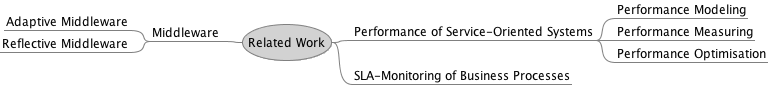
\includegraphics[width=\textwidth]{img/related_work_map.png}
	\caption{Related Work}
	\label{fig:related_work_map}
\end{figure}
\section{Performance of Service-Oriented Systems}
\citet{OBrien:2007fk} argue that the introduction of an SOA generally has a negative impact on the performance of the system. They identify the following key aspects responsible for the performance degradation:
\begin{itemize}
	\item \textbf{Network communication}\\
	Service provider and service consumer need to communicate over a network, which usually does not offer a deterministic latency.
	\item \textbf{Lookup of services in a directory}\\
	The lookup of a service provider in a directory increases the total transaction time of a service request.
	\item \textbf{Interoperability of services on different plattforms}\\
	The interoperability of services on different platforms is realized by a middleware which handles the whole communication. The needed marshalling and unmarshalling of data adds a performance overhead to the communication.
	\item \textbf{Usage of standard messaging formats}\\
	The usage of a standard message format, like XML, increases the processing time of a service due to parsing, validation and transformation of messages. An XML message can be 10 to 20 times larger than the binary representation which increases the the transport time of the message over the network.
\end{itemize}
In another paper, \citet{OBrien:2008uq} state that the performance issues of an SOA are caused by:
\begin{itemize}
	\item Overhead of XML
	\item Implementation of composite services
	\item Service orchestration
	\item Service invocation
	\item Resources, e.g. threads, CPUs
	\item Resource models, e.g. virtualization
\end{itemize}
The authors suggest that it is vital to consider performance aspects early in the development lifecycle, which can be supported by using an SOA performance model.

\citet{Woodall:2007kx} describe in their paper the challenges they encountered when analysing a performance problem of a concrete Service-Oriented System:
\begin{itemize}
	\item Physical distribution of services
	\item Continual use of services by local users or developers during the performance investigation
	\item Heterogeneity of the underlying service software plattform
\end{itemize}

\section{Performance Measuring}
Performance measuring is applied to evaluate if an implemented system meets its performance requirements and to spot possible performance problems.

\citet{Her:2007qf} propose the following set of metrics for measuring the performance of a service-oriented system:
\begin{itemize}
	\item \textbf{Service response time}\\
	Elapsed time between the end of request to service and the beginning of the response of the service. This metric is further split in 20 sub-metrics such as message processing time, service composition time and service discovery time.
	\item \textbf{Think time}\\
	Elapsed time between the end of a response generated by a service and the beginning of a response of an end user.
	\item \textbf{Service tournaround time}\\
	Time needed to get the result from a group of related activities within a transaction.
	\item \textbf{Throughput}\\
	Number of requests served at a given period of time. The authors distinguish between the throughput of a service and the throughput of a business process.
\end{itemize}

In their work, \citeauthor{Henjes:2006nx} investigated the throughput performance of the JMS server FioranaMQ, SunMQ and WebsphereMQ. The authors came to the following conclusion (\citet{Henjes:2006nx} and \citet{Menth:2006qe}):
\begin{itemize}
	\item Message persistence reduces the throughput significantly.
	\item Message replication increases the overall throughput of the server.
	\item Throughput is limited either by the processing logic for small messages or by the transmission capacity for large messages.
	\item Filtering reduces the throughput significantly.
\end{itemize}

\citet{Chen:2004cr} propose that the following performance metrics should be used to evaluate a JMS server:
\begin{itemize}
	\item Maximum sustainable throughput
	\item Latency
	\item Elapsed time taken to send batches messages
	\item Persistent message loss after recovery
\end{itemize}
The authors state that ``although messaging latency is easy to understand, it is difficult to measure precisely in a distributed environment without synchronised high- precision clocks.'' They discovered that latencies increase with increasing message sizes.

SPECjms2007 is a standard benchmark for the evaluation of Message-Oriented Middleware platforms using JMS \citep{Sachs:2009rr}. It provides a flexible performance analysis framework for tailoring the workload to specific user requirements. According to \citet{sachs2007designing}, the workload of the SPECjms2007 benchmark has to meet the following requirements:
\begin{itemize}
	\item \textbf{Representativeness}\\
	The workload should reflect how the messaging platform is used in typical user scenarios.
	\item \textbf{Comprehensiveness}\\
	The workload should incorporate all platform features typically used in JMS application including publish/subscript and point-to-point messaging.
	\item \textbf{Focus}\\
	The workload should focus on measuring the performance of the messaging middleware and should minimize the impact of other components and services.
	\item \textbf{Configurability}\\
	It should be possible to configure the workload to meet the requirements of the user.
	\item \textbf{Scalability}\\
	It should be possible to scale the workload by the number of destinations with a fixed traffic per destination or by increasing the traffic with a fixed set of destinations.
\end{itemize}
\section{Performance Optimisation}
Most of the work that aims to optimise the performance of service-oriented systems is done in the area of Web Services since it is a common technology to implement a SOA.

In particular, various approaches have been proposed to optimise the performance of SOAP, the standard protocol for Web Service communication. This includes approaches for optimising the processing of SOAP messages (see for example \citet{Abu-Ghazaleh:2005bs}, \citet{Suzumura:2005fv} and \citet{Ng:2006kl}), compression of SOAP messages (see for example \citet{Estrella:2008dz} and \citet{Ng:2005qa}) and caching (see for example \citet{andresen2004lye} and \citet{Devaram:2003fu}). A survey of the current approaches to improve the performance of SOAP can be found in \cite{Tekli:2012bh}.

\citet{Wichaiwong:2007oq} propose an approach to transfer bulk data between web services per FTP. The SOAP messages transferred between the web services would only contain the necessary details how to download the corresponding data from an FTP server since this protocol is optimized for transferring huge files. This approach solves the technical aspect of efficiently transferring the input and output data but does not pose any solutions how to implement loose coupling and how to integrate heterogeneous technologies, the fundamental means of an SOA to improve the flexibility of an application landscape.

Data-Grey-Box Web Services are an approach to transfer bulk data between Web Services \citep{Habich:2007ij}. Instead of transferring the data wrapped in SOAP messages, it is transferred using an external data layer. For example when using database systems as data layer, this facilitates the use of special data transfer methods such ETL (Extract, Transform, Load) to transport the data between the database of the service requestor and the database of the Web service. The data transfer is transparent for both service participants in this case. The approach includes an extension of the Web service interface with properties describing the data aspects. Compared to the SOAP approach, the authors measured a speedup of up to 16 using their proposed approach. To allow the composition and execution of Data-Grey-Box Web services,  \citet{Habich:kl} developed BPEL data transitions to explicitly specify data flows in BPEL processes.

\cite{Zhuang:2012qf} propose three tuning strategies to improve the performance of \ac{JMS} for cloud-based applications.
\begin{enumerate}
	\item When using persistent mode for reliable messaging the storage block size should be matched with the message size to maximise message throughput.
	\item Applying distributed persistent stores by configuring multiple JMS destinations to achieve parallel processing
	\item Choosing appropriate storage profiles such as RAID-1
\end{enumerate}

MPAB (Massively Parallel Application Bus) is an ESB-oriented messaging bus used for the integration of business applications \citep{Benosman:2012zr}. The main principle of MPAB is to fragment an application into parallel software processing units, called SPU. Every SPU is connected to an Application Bus Multiplexor (ABM) through an interface called Application Bus Terminal (ABT). The Application Bus Multiplexor manages the resources shared across the host system and communicates with other ABM using TCP/IP. The Application Bus Terminal contains all the resources needed by SPU to communicate with its ABM. A performance evaluation of MPAB shows that it achieves a lower response time compared to the open source ESBs Fuse, Mule and Petals.

Some research has been done to add real-time capabalities to ESB or messaging middleware. \cite{Garces-Erice:2009kx} proposes an architecture for a real-time messaging middleware based on an Enterprise Service Bus. It consists of an event scheduler, a \ac{JMS}-like API and a communication subsystem. While fulfilling real-time requirements, the middleware also supports already deployed infrastructure.

In their paper, \cite{Xia:2011rt} suggest a real-time ESB model by extending the JBI specification with semantics for priority and time restrictions and modules for flow control and bandwith allocation. The proposed system is able to dynamically allocate bandwidth according to business requirements.

Tempo is a real-time messaging system written in Java that can be used on either a real-time or non-real-time architecture \citep{Bauer:2008fk}. The authors, Bauer et al., state that existing messaging systems are designed for transactional processing and therefore not appropriate for applications with with stringent requirements of low latency with high throughtput. The main principle of Tempo is to use an independent queuing system for each topic. Ressources are partitioned between these queueing systems by a messaging scheduler using a time-base credit scheduling mechanism. In a test environment, Tempo is able to process more than 100.000 messages per second with a maximum latency of less than 120 milliseconds.

\cite{Haesen:2008ve} distinguishes between two types of data granularity:
\begin{itemize}
	\item \textbf{Input data granularity}\\
	Data that is sent to a component
	\item \textbf{Output data granularity}\\
	Data that is returned by a component
\end{itemize}
The authors state that a coarse-grained data granularity reduces the communication overhead, since the number of network transfers is decreased.
``Especially in the case of Web services, this overhead is high since asynchronous messaging requires multiple queuing operations and numerous XML transformations''.

\section{Self-Adaptive Software Systems}

\begin{itemize}
	\item Definition Self-Adaptive Software
	\item Reference Architectures for self-adaptive software systems
	\begin{itemize}
		\item Three Layer Architecture Model for Self-Management \citep{Kramer:2007ff}
		\item Conceptual Architecture for Self-Adaptive Software Systems \citep{Andersson:2009bq}
		\item Mape-K \citep{Group:2005ug}
	\end{itemize}
	\item Self-adaptive properties
	\begin{itemize}
		\item Automatic Workarounds
	\end{itemize}
	\item Self-adaptive middleware
	\begin{itemize}
		\item Self-adaptive \ac{SOA}
		\item Self-adaptive \ac{ESB}
	\end{itemize}
	\item Self-adaptive frameworks
	\begin{itemize}
		\item Rainbow framework
		\item PLASTIC
		\item Javeleon
		\item JavAdaptor
		\item ArchJava
	\end{itemize}
\end{itemize}

\subsection{Definition}
Self-Adaptive Software is a ``a closed-loop system with a feedback loop aiming to adjust itself to changes during its operation'' \citep{Salehie:2009pi}. These changes can originate from internal causes of the system (the system's self) or from the context of the system.

\citet{Laddaga:2008ff} provides a definition for self-adaptive software: ``Self-adaptive software evaluates its own behavior and changes behavior when the evaluation indicates that it is not accomplishing what the software is intended to do, or when better functionality or performance is possible.'' 

Another definition is given by \citet{Oreizy:1999lh}: ``Self-adaptive software modifies its own behavior in response to changes in its operating environment. By operating environment, we mean anything observable by the software system, such as end-user input, external hardware devices and sensors, or program instrumentation.''

\cite{Salehie:2009pi} describe the following properties (also called self-* properties) of a self-adaptive system:
\begin{itemize}
	\item \textbf{Self-configuring}\\
	The system is able to reconfigure itself in response to changes.
	\item \textbf{Self-healing}\\
	The system is able to discover, diagnose and react on failures.
	\item \textbf{Self-optimizing}\\
	The system is able to manage performance and resource allocation to meet different performance requirements.
	\item \textbf{Self-protecting}\\
	The system is able to detect security breaches and to recover from them.
\end{itemize}

More general self-* properties are described as:
\begin{itemize}
	\item \textbf{Self-Awareness}\\
	The system is aware of its self states and behaviours.
	\item \textbf{Context-Awareness}\\
	The system is aware of its context.
\end{itemize}

\section{Self-Adaptive Middleware}

\citet{Duran-Limon:2004mi} argue that ``the moste adequate level and natural locus for applying adaption is at the middleware level''. Adaption at the operating system level is platform-dependent and changes at this level affect every application running on the same node. On the other hand, adaption at application level assigns the responsibility to the developer and is also not reusable.

\citet{Lee:2009vn} propose an adaptive, general-purpose runtime infrastructure for effective resource management of the infrastructure. Their approach is comprised of three components:
\begin{enumerate}
	\item dynamic performance prediction
	\item adaptive intra-site performance management
	\item adaptive inter-site resource management
\end{enumerate}

The runtime infrastructure is able to choose from a set of performance predictions for a given service and to dynamically choose the most appropriate prediction over time by using the prediction history of the service.

AutoGlobe \citep{Gmach:2008vo} provides a platform for adaptive resource management comprised of 
\begin{enumerate}
	\item Static resource management
	\item Dynamic resource management
	\item Adaptive control of Service Level Agreements (SLA)
\end{enumerate}
Static resource management optimises the allocation of services to computing resources and is based on on automatically detected service utilisation patterns. Dynamic resource management uses a fuzzy controller to handle exceptional situations at runtime. The Adaptive control of Service Level Agreements schedules service requests depending on their SLA agreement.

The coBRA framework proposed by \citet{Irmert:2008nx} is an approach to replace service implementations at runtime as a foundation for self-adaptive applications. The framework facilitates the replacement of software components to switch the implementation of a service with the interface of the service staying the same.

DREAM (Dynamic Reflective Asynchronous Middleware) \citep{Leclercq:2004ly} is a component-based framework for the construction of reflective Message-Oriented Middleware. Reflective middleware ``refers to the use of a causally connected self-presentation to support the inspection and adaption of the middleware system'' \citep{Kon:2002fu}. DREAM is based on FRACTAL, a generic component framework and supports various asynchronous communication paradigms such as message passing, event-reaction and publish/subscribe. DREAM facilitates the construction and configuration of Message-Oriented Middleware from a library of components such as message queues, filters, routers and aggregators, which can be assembled either at deploy-time or runtime.
\section{SLA-Monitoring of Business Processes}
The SECMOL framework (Service Centric Monitoring Language), developed by \citet{Guinea:2009fk}, allows to monitor the quality of service constraints of BPEL processes. It is comprised of three components. Data Collectors for capturing data, Data Analyzers for analysing the captured data and the Monitoring Manager for coordinating the monitoring process. SECMOL also defines a XML-based monitoring specification, which consists of monitoring policies that specify how the monitoring should be done and monitoring rules that express the quality of service properties the system needs to satisfy.

\citet{Duc:2009kx} argue that a monitoring middleware component should fulfill the following requirements:
\begin{itemize}
	\item \textbf{Coherency of data}\\
	All data used in one decision must reflect the same state of the system.
	\item \textbf{Flexibility in data access}\\
	Every monitored service provider should be able to respond using its own measurement units. This should be transparent for the client using the monitoring data.
	\item \textbf{Performance in data access}\\
	The monitoring should have the slightest possible impact on the performance of the business process.
	\item \textbf{Network usage optimisation}\\
	The transmission of monitoring data should have the slightest possible impact on the network performance.
\end{itemize}
The authors propose M4ABP (Monitoring for Adaptive Business Process), a distributed monitoring and data delivery middleware subsystem, which implements these requirements.

SALMon \citep{Ameller:2008zr} is a system for monitoring the services of an SOA for Service Level Agreement violations. It is itself implemented as an service-oriented system and consists of the following services:
\begin{itemize}
	\item \textbf{Monitor}\\
	The Monitor service collects the monitoring data from components called Measure Instruments that are instantiated in each monitored service. 
	\item \textbf{Analyzer}\\
	The Analyzer service manages the Monitor service and checks for Service Level Agreement violations of the monitored services.
	\item \textbf{Decision Maker}\\
	The Decision Maker service is able to select an action to solve the SLA violation. The appropriate action for a specific SLA violation is stored in a repository.
\end{itemize}
The attributes measured by SALMon are taken from an ISO/IEC 9126-1-based quality model.

\citet{Textor:2009vn} propose an approach to map implementation level monitoring data to business level activities. Non-functional constraints are specified on a workflow model in the modelling phase. Additionally, an instrumentation model is used to specify the instrumentation points of the application. At runtime, the monitoring data of the system is mapped to the workflow model. 
The monitoring data is received by a component called ConstraintMonitor, which evaluates and validates the constraints specified in the workflow model.

\citet{Wetzstein:2009uq} present a framework to monitor and analyse the factors that influence the performance of WS-BPEL processes. The authors distinguish between PPM (Process Performance Metrics) and QoS (Quality of Service) metrics, which influence the Key Performance Indicators (KPI) of business processes. PPMs are based on process runtime events, that are published by the WS-BPEL runtime engine, for example the ``number of orders which can be served as inhouse stock''. QoS metrics are technical parameters of the underlying services that implement the business process, for example the response time and availability of a service. KPIs are based on business goals, for example ``order fulfillment lead time < 3''. The proposed framework monitors KPIs, PPMs and QoS metrics at runtime, which are modeled in a Process Metrics Definition Model (PMDM). These collected metrics can then be used to perform a dependency analysis of the influential factors of a KPI using machine learning techniques to construct dependency trees.

iBOM \citep{Castellanos:2005fk} is a platform to analyse, manage and optimise business operations based on business goals. Optimisations are performed by using simulation techniques. iBom simulates different configurations of a business process to identify the configuration that best meets the business goals. First, the user needs to define the optimisation metric and constraints on this metric and on the resources. The configuration candidates are then either computed by iBOM using different resource allocations of the given configuration within the defined constraints or are provided by the user in the form of a process model. 

\section{Software Performance Engineering}

\begin{itemize}
	\item \ac{SPE} is a ``method for constructing software systems to meet performance objectives'' \citep{Smith:1990aa}.
	\item The process begins early in the software lifecycle
	\item Uses quantitative methods to indentify designs that meet the performance requirements and to dismiss those that are likely to miss them.
	\item \ac{SPE} is continued during detailed design, implementation test and operation to predict and manage the performance of a software system and to monitor and report the actual performance fo the system.
	\item \ac{SPE} methods include performance data collection, quantitative analysis techniques, prediction strategies, management of uncertainties, data presentation and tracking, model verification and validation, critical success factors, and performance design principles. 
	\item \citep{Woodside:2007aa} differentiates between two general approaches
	\begin{itemize}
		\item measurement-based
		\begin{itemize}
			\item testing, diagnosis and tuning late in the development cycle, when the system is already implemented and can be run and tested.
		\end{itemize}
		\item model-based
		\begin{itemize}
			\item creates performance models and uses quantitative results from these models early in the development cycle to predict the performance of the system and to adjust the architecture of the system to meet its performance requirements.
		\end{itemize}
	\end{itemize}
\end{itemize}

\begin{itemize}
	\item Best Practices for Software Performance Engineering \citep{Smith:2003aa}
\end{itemize}

\section{Summary}

\begin{itemize}
  \item Performance optimization is done at the transport layer (XML, Messaging)
\end{itemize}

Most of the work done in the field of performance of service-oriented systems involves performance aspects of Web Services including the SOAP standard. This includes performance modeling, performance measuring and performance optimisation. 

Approaches to optimise the transfer of bulk data of Web services, as proposed by \citet{Wichaiwong:2007oq} and  \citet{Habich:2007ij} deliver an overall better performance than using SOAP. However, like a traditional batch-processing system using file- or database-based integration, they are not able to reduce the latency and thus cannot deliver near-time processing of bulk data.

Current self-adapting middleware platforms, like the AutoGlobe platform \citep{Gmach:2008vo}, are focused on adaptive resource management to dynamically allocate services to computing nodes or to replace service implementations at runtime, as proposed by the coBRA framework \citep{Irmert:2008nx}.

Work on SLA-monitoring of business processes proposes different approaches to monitor the compliance of a business process to Service Level Agreements, which include the end-to-end latency and throughput of the business process. However, they do not propose any solutions for improving the end-to-end latency in order to provide near-time processing of bulk data.

The research project presented in this report proposes an adaptive middleware to reduce the latency of a system for bulk data processing by dynamically adjusting the data granularity at runtime based on the current throughput and the minimum acceptable throughput of the system. To the best of our knowledge, this is a novel approach which has not yet been discussed in current literature.